    % mostly DONE exept 2 TODO , address when writing future and conclusion!

    This part uses the previously introduced library to implement DAGA in the cothority framework\sidecite{dedis_scalable_nodate}.
    \newline\noindent
    Cothority is a DEDIS project that \blockquote{
        provides a framework for development, analysis, and deployment of decentralized, distributed (cryptographic) protocols.
        A given set of servers running these protocols is referred to as a collective authority or cothority.
        Individual servers are called cothority servers or conodes\footnotemark[\thefootnote]
    }.%\newline
    The following figure depicts an high-level overview of the new DAGA cothority that will be subsequently
    described.
    \begin{figure}% or marginfigure scale=0.45/or reduce cothority and give more room to part below
        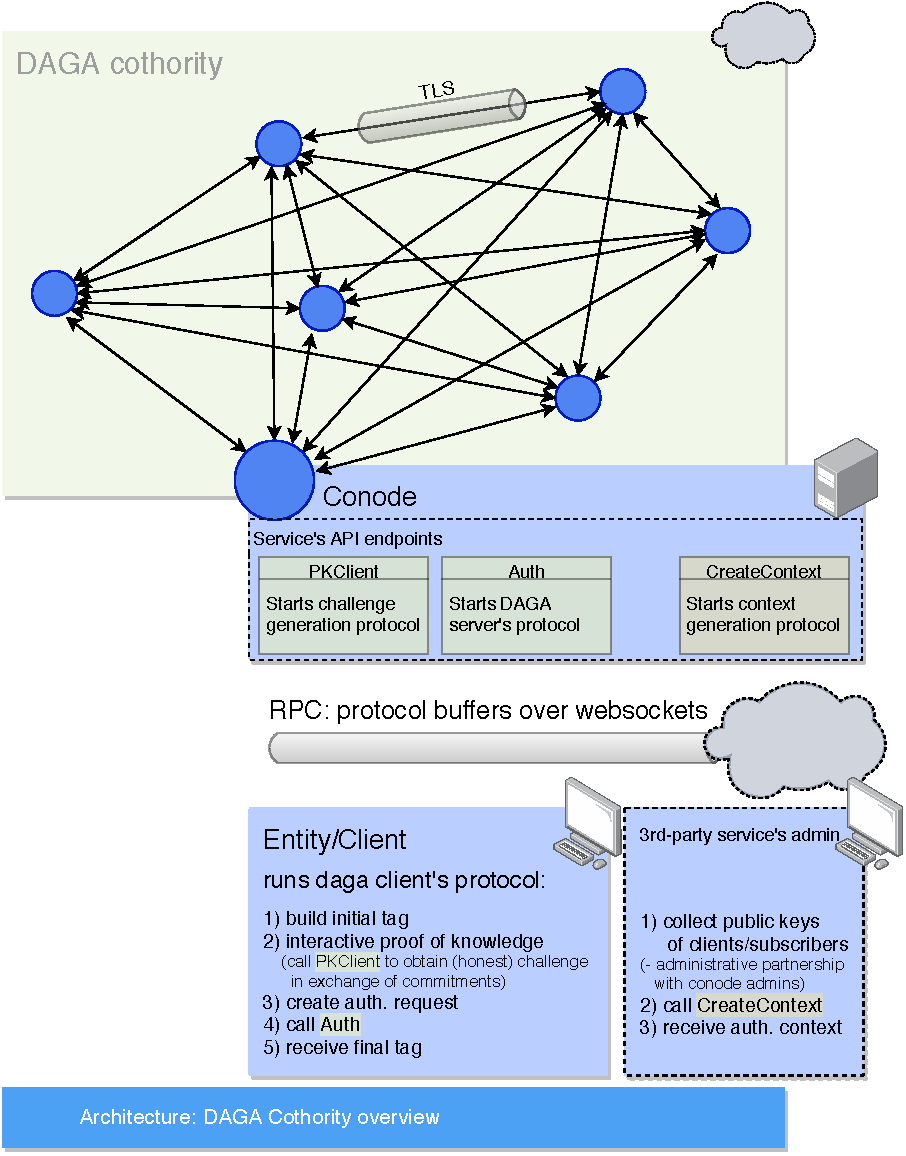
\includegraphics[scale=0.7]{images/dagacothority.pdf}
        \caption{high level overview of DAGA in the cothority framework}
        \label{fig:dagacothority}
    \end{figure}

    \subsubsection{Context Creation}
    As said in the background chapter, every party needs to have access to a public (in the "not sensitive" sense)
    authentication context\sidenote{see section~\ref{subsubsec:dagacontext}} before being able to do anything.
    To create such context, the protocol described in~\cite[Sect.~4.7.3]{syta_identity_2015} was implemented. % TODO stress somehow that this is new ?

    A client can (typically an admin of a 3rd-party service)
    create a context by:
    \begin{enumerate}[leftmargin=!,itemsep=-1ex]
        \item Gathering the long-term public keys\sidenote {
        To do so it is envisioned to offer tools allowing to scrap them out of a POP\cite{borge_proof--personhood:_2017}
        party transcript for instance,
        but the admin is free to collect them by any mean that fits its agenda.
        } of the \emph{group} members (or entities, typically the subscribers of the service).

        \item building a cothority by establishing individually and administratively partnerships with the admins that run
        DAGA enabled conodes. (but we can imagine "open access" conodes) and creating a roster\sidenote{
        a structure describing basically how to reach them and communicate securely with them (public keys)
        } out of the  process.

        \item finally sending an authenticated CreateContext request (containing the keys and roster) to a random conode in the roster.
    \end{enumerate}

    Then the conode receiving the request checks first if it has a matching partnership before initiating a new instance of
    the context generation protocol, with the other nodes listed in the roster as partners.
    During the protocol run, all other conodes will check in their turn if they accept the request before acceding to the
    request of the leader and helping it building the context.
    At the end of a successful protocol run (where nothing strange has been detected by any node), the new context is sent
    back to the client and every node will start serving the newly created DAGA context.\sidenote{
    or said differently, accepting authentication requests under the context, and hence establishing effectively a new
    \emph{collective authority} for the context by doing so.
    }

    \smalltitle{Current state:}
    As currently implemented, each conode can serve multiple different contexts at once
    (each with possibly different daga server identities/public keys)
    % TODO ? one key one purpose, dissociate daga service from conode/onet internals choices of keys etc..
    % node-node channels are authenticated using keys in roster which is tied to authentication context
    and at the end of each context creation the state is persisted in
    a bbolt database, allowing a node to retrieve it after a potential shutdown or crash without destroying permanently the cothority
    and/or forcing everyone to rebuild a context.

    However there are currently no facilities/boilerplate to manage and conduct the administrative partnerships that was mentioned in the
    described scenario nor to authenticate the 3rd-party services admins, hence currently the conodes are "open access" DAGA nodes.
    Still the service and protocol were implemented while keeping those ideas in mind and already have places to check such things,
    making the addition straightforward.\sidenote{
        Have a look at the dagacothority/service/service.go
    }
    One of the ideas would be, interestingly, to reuse DAGA for that purpose, we can imagine that we define administratively/offline a
    context whose members are the people that have a partnership with the conode that allow them to create contexts (~similar to authenticated darcs).
    Then a running cothority (serving the context) and containing the conode, authenticates the request.
%    => the node is convinced that the "remote now anon 3rd-party service admin" has the right to create new contexts
%    => (+) KISS, can use only DAGA, no need to use alien protocols and things like openPGP or DARC management etc..
%    => (+) ~"eat your own food" preserve 3rd-party admin privacy, don't throw out of the window our own goals and advices on the separation of authentication and identification etc..
%    => the thing now becomes: offering ways to manage the partnerships and setup those partnership contexts.
%    chicken and egg problem but now we can decide to bootstrap them differently using whatever means we want
%    (a cli app ? + administrative context loaded from known location at setup time)

    %TODO ref% FIXME cross ref to Future where I'll talk about the things envisioned for the auth. !!

    As seen the DAGA cothority was designed such that every conode retains completely its free-will,
    each conode is independent and tied only by the contexts it serves to form possibly multiple cothorities with possibly
    different partners.
    Finally quoting~\cite{syta_identity_2015} those DAGA enabled conodes are expected to be \blockquote{
        deployed by a federation of organizations wishing to support responsible forms of anonymous participation (...),
        anonymity system providers such as the Tor project, non-profit organizations whose aim is to further online privacy
        and anonymity, or even for-profit organization desiring strong guarantees and large anonymity sets for their clients.
    }

    \subsubsection{Authentication and \(\Sigma\)-Protocol}
    \label{subsubsec:sigmaprotocol}

    A client having in possession a suitable authentication context
    can authenticate itself to the DAGA cothority by sending its authentication message to the \emph{Auth} endpoint of a random conode.

    As already described in section~\ref{subsubsec:dagaauth}, to build such an authentication message, the client
    has to conduct a zero-knowledge proof of knowledge with the cothority at the verifying side.
    To do so it will call the \emph{PKClient} endpoint of a random conode to request a challenge in exchange of commitments.

    Since the proof in question is of the \(\Sigma\)-protocol kind, the zero-knowledge property\sidenote{
    and hence the anonymity and deniability properties of DAGA
    } holds only if the verifiers (thus the challenge) are honest\sidenote{(special HVZK property)}.
    Hence we need to have the servers \blockquote{
    collectively generate \(c_s\) [(the challenge)] so that each server, which would include at least
    one honest server, contributes its randomness towards \(c_s\).
    }\cite{syta_identity_2015}
    Moreover if the prover can predict the challenge (maybe with the help of some dishonest servers),
    it will allow it to cheat by crafting its first move (the commitments) using the verification formula
    or put differently, by abusing the HVZK proof structure and using the "simulator + rewind verifier" approach.
    % TODOs, check what aboout the space of the challenge, remember having read sommewhere that it should not be too large
    % for the ZKness to hold...=> if thats the case then here is a shady thing in daga

    \noindent
    To summarize the distributed challenge generation protocol has two main purposes:
    \begin{enumerate}
        \item the obvious one : make the "verifier"(cothority) honest to keep the proof zero-knowledge.
        this is solved by the fact that we assume an anytrust setting, at least one honest server will contribute its randomness to the challenge.
        \item the less obvious one: convince individually the servers that the challenge is honest
        (they trust themselves to add their randomness to it) and that the client and other servers cannot collude and cheat.
    \end{enumerate}
    Hence at the end both the honest client and the honest server are ensured of the randomness and "honesty" of the cothority as a whole.

    % TIE to commitments, state etc..
    Additionally, the proof being interactive\sidenote{in order to offer the deniability property of DAGA},
    it convinces only the participants.
    As a consequence, if the servers want to verify it later (Auth endpoint) based only on the transcript embedded in the authentication message\sidenote{
        That's how DAGA is described in~\cite{syta_identity_2015},
    }, additional care and mechanisms should be put in place.
    Indeed if nothing is done (as it was the case with the previous implementation\cite{villard_deniable_2017}) the prover
    can cheat using the same technique described above.\newline
    There are two approaches to prevent this from happening:
    \begin{enumerate}
        \item keep state (commitments and challenge) between the \emph{PKClient} and \emph{Auth} requests at each node,
                and rely only on it to verify the proof.
                This approach was chosen by~\sidecite{wolinsy_daga_2014}
        \item or avoid by following the "keep state in clients" motto of RESTFul services.
    \end{enumerate}

    We chose the second option, and implemented it by having the servers tie the challenge to the commitments by
    each issuing a signature on \(challenge||commitment\) instead of only challenge at the \emph{PKClient} step.
    This way, when the client calls later the \emph{Auth} endpoint, the servers can individually verify that the challenge
    and commitments have not been altered by verifying their own signatures\sidenote{
        the signature ties the challenge to the commitments and at the same time protects authenticity and integrity of the pair
    }.

    % TODO ? - verifier extracting secret, would be the right place, ...
    %(if proof run 2 times with same commitments, i.e. abusing special soundness proof, using "extractor + rewind prover" approach => PRNG must be properly setup !!)
    % careful with rndgen, special soundness property allows people with 2 transcripts such as as malicious server to extract
    % client secret key (only if prover rewound,  same t ==> means need to be sure that random properly working !! => care in cloud setup if not proper source of entropy)
    % this is done correctly by using golang's crypto.rand that should do the job

%    % FIXME: here with new title thoughts/etc. or future/conclusion, see when writing future
%    TODO
%    at one point I investigated the possibility to use randherd to generate the challenges
%    => not done because :
%    1) time, first simpler min viable approach
%    2) add a dependency to daga, tie to implementation in cothority framework => need to maintain 2 things (kyber daga need to have things related to building challenge)
%    3) not sure how to tie the resulting challenge to commitments in a way that convince everyone that nobody is cheating
%    see later, now each server signs cs||commitments at the end (and is convinced is random by construction, add his own randomness)
%    but at the end of randherd, client of randherd call (say leader of daga challenge generation)
%    obtain decentralized honest publicly verifiable randomness ? but how can we tie it to the commitments at all servers ?
%    say that it is the client while building proof that request the challenge via randherd (same cothority for randherd + daga)
%    as before problem is servers' don't have a chance to tie the challenge to the commitments to prevent prover cheating (see proof)
%    => fallback to first option manage request state in servers
%    since time was short, idea dropped/postponed



